\subsection{Mô tả kiến trúc hệ thống}
\begin{figure}[h!]
    \centering
    \setlength{\abovecaptionskip}{10pt}
    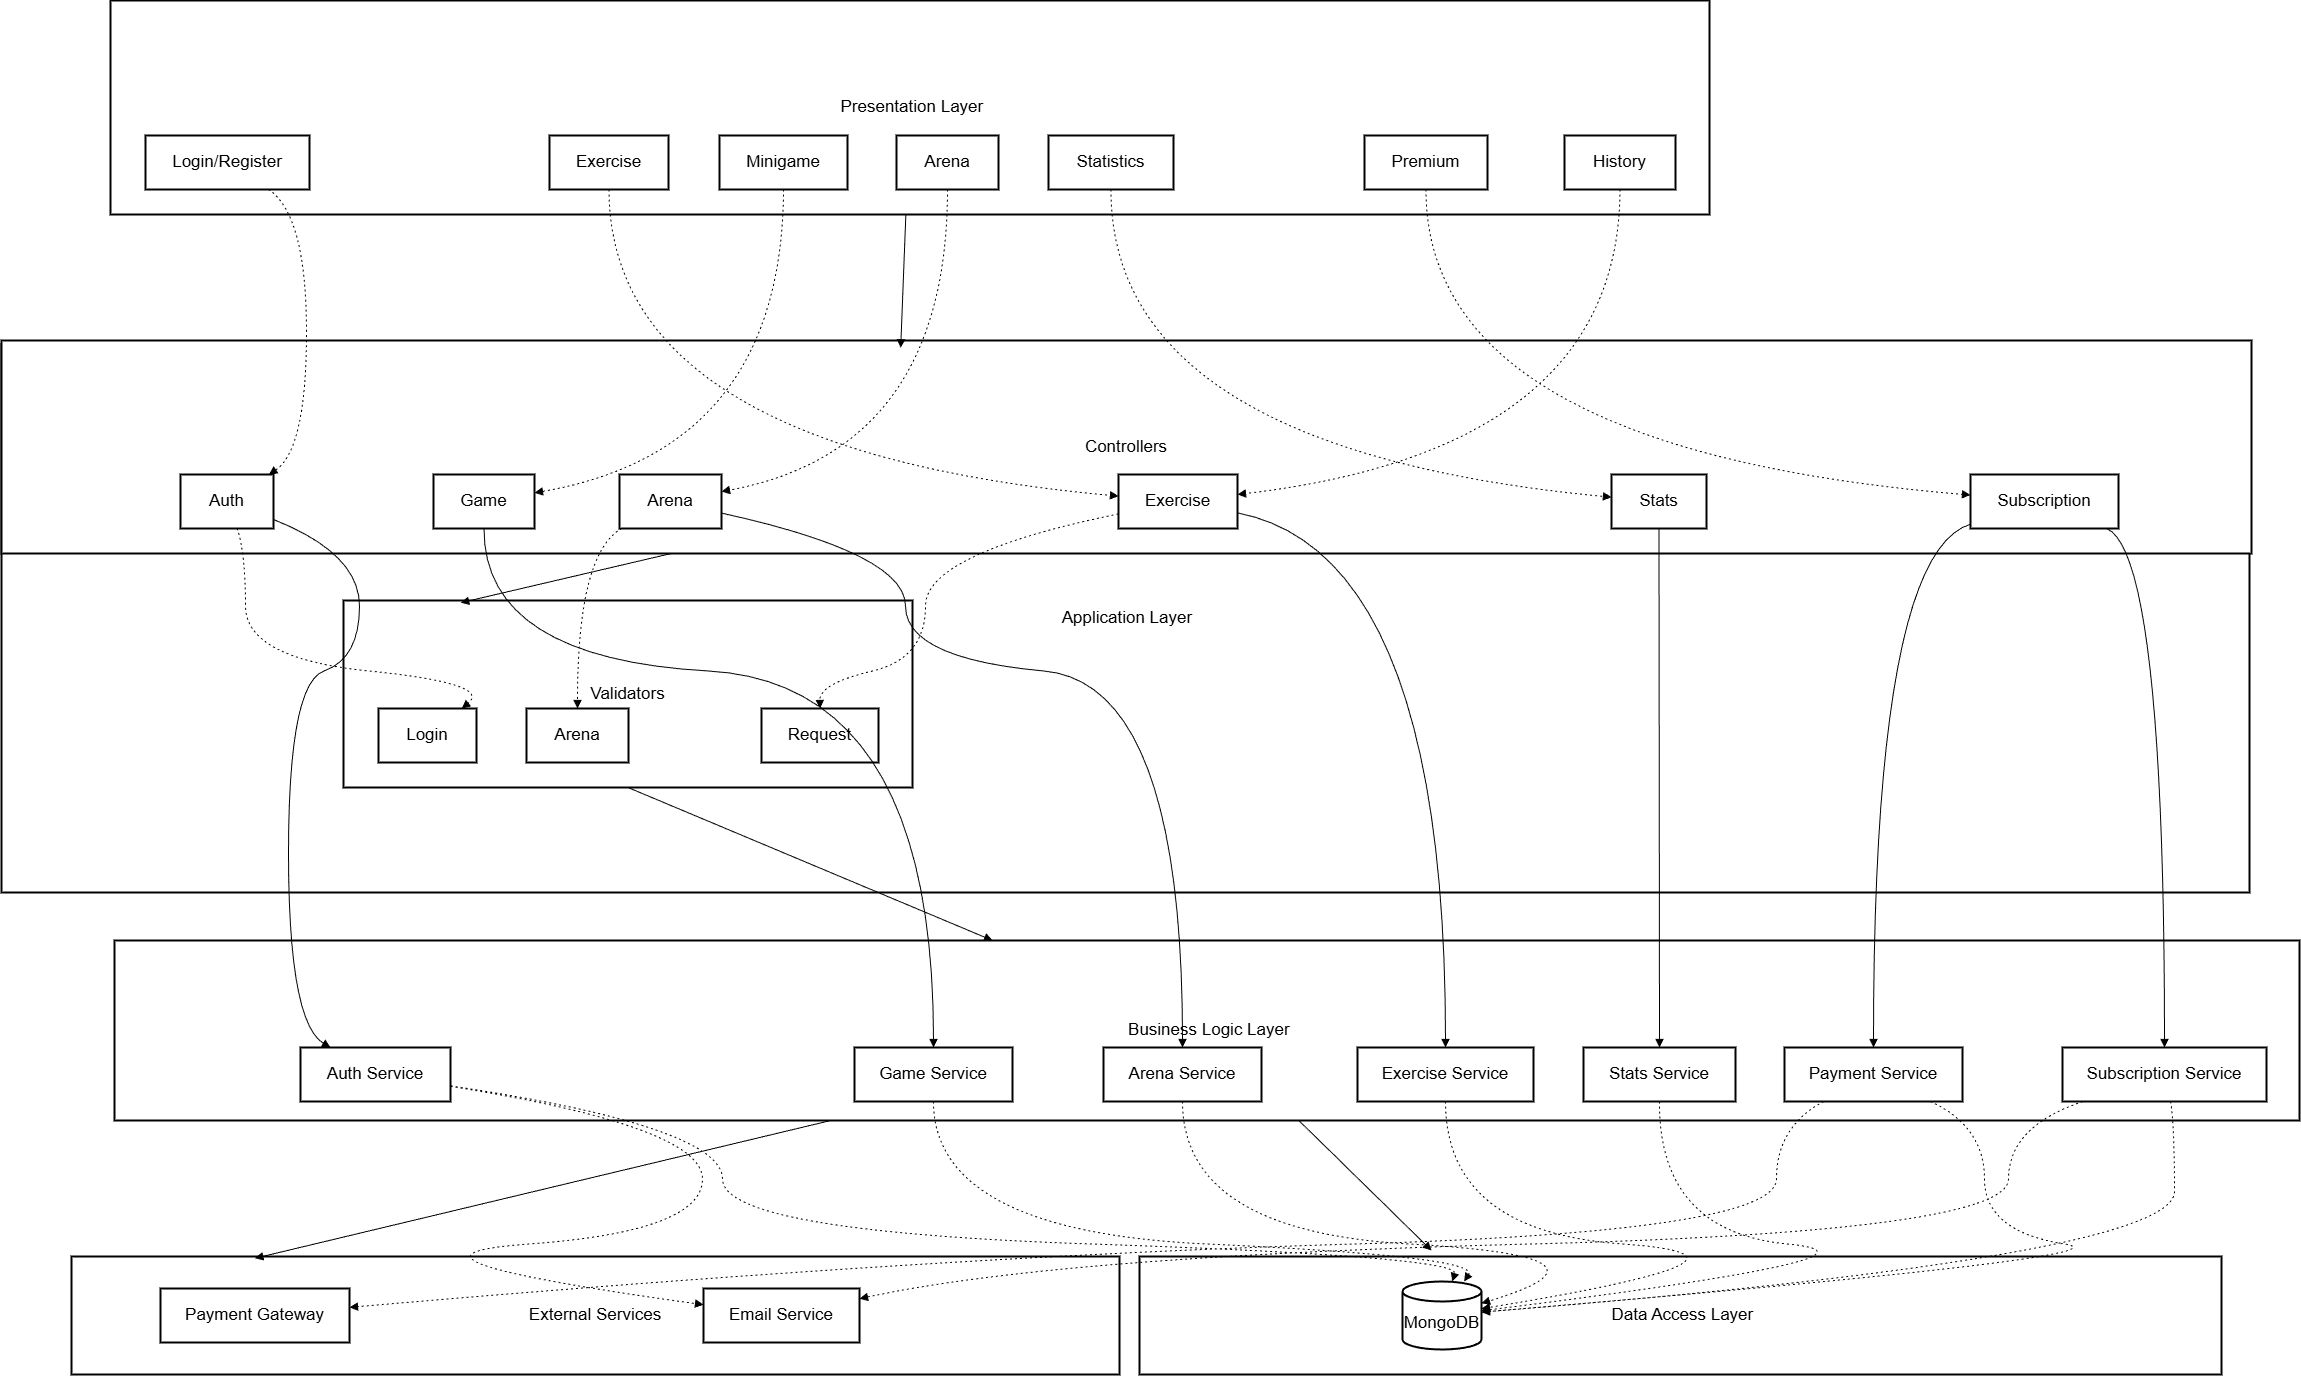
\includegraphics[width=\textwidth]{Image/Untitled Diagram-Page-16.drawio.png}
    \caption{Sơ đồ kiến trúc tổng thể của hệ thống}
    \label{fig:system-architecture}
\end{figure}


Hệ thống được thiết kế theo mô hình kiến trúc nhiều tầng (layered architecture), nhằm tách biệt rõ ràng giữa giao diện người dùng, xử lý nghiệp vụ và truy cập dữ liệu, từ đó tăng khả năng mở rộng, bảo trì và kiểm thử.
Hệ thống được thiết kế theo mô hình kiến trúc nhiều tầng (layered architecture), nhằm tách biệt rõ ràng giữa giao diện người dùng, xử lý nghiệp vụ và truy cập dữ liệu, từ đó tăng khả năng mở rộng, bảo trì và kiểm thử.

\subsubsection{Presentation Layer}
Tầng trình bày chịu trách nhiệm tương tác trực tiếp với người dùng, bao gồm các màn hình và chức năng như \textit{Login/Register}, \textit{Exercise}, \textit{Minigame}, \textit{Arena}, \textit{Statistics} và \textit{History}.  
Các thành phần này không xử lý logic nghiệp vụ mà chỉ gửi yêu cầu và hiển thị kết quả trả về từ tầng Controller.

\subsubsection{Controller Layer}
Tầng Controller đóng vai trò trung gian giữa Presentation Layer và Application Layer.  
Mỗi controller (Auth, Game, Arena, Exercise, Stats) tiếp nhận request từ giao diện người dùng, thực hiện điều phối luồng xử lý và gọi các thành phần nghiệp vụ tương ứng.  
Trước khi chuyển tiếp yêu cầu, controller sử dụng các \textit{Validators} để kiểm tra dữ liệu đầu vào nhằm đảm bảo tính hợp lệ và an toàn.

\subsubsection{Application Layer}
Tầng ứng dụng chịu trách nhiệm điều phối logic ở mức cao, kết nối giữa controller và các service nghiệp vụ.  
Tại tầng này, hệ thống đảm bảo các use case được thực thi đúng trình tự, không phụ thuộc trực tiếp vào chi tiết cài đặt của tầng Business Logic hay Data Access.

\subsubsection{Business Logic Layer}
Tầng nghiệp vụ chứa các service cốt lõi của hệ thống, bao gồm \textit{Auth Service}, \textit{Game Service}, \textit{Arena Service}, \textit{Exercise Service}, \textit{Stats Service}, \textit{Payment Service} và \textit{Subscription Service}.  
Mỗi service chịu trách nhiệm xử lý một nhóm nghiệp vụ cụ thể, đóng gói các quy tắc nghiệp vụ và đảm bảo tính nhất quán của dữ liệu.  
Các service này có thể giao tiếp với nhau khi cần thiết, đồng thời tương tác với các dịch vụ bên ngoài.

\subsubsection{Data Access Layer}
Tầng truy cập dữ liệu chịu trách nhiệm lưu trữ và truy xuất dữ liệu từ cơ sở dữ liệu MongoDB.  
Tất cả các thao tác với dữ liệu đều được thực hiện thông qua tầng này, giúp cô lập logic nghiệp vụ khỏi chi tiết cài đặt của hệ quản trị cơ sở dữ liệu.

\subsubsection{External Services}
Hệ thống tích hợp với các dịch vụ bên ngoài như \textit{Payment Gateway} để xử lý thanh toán và \textit{Email Service} để gửi thông báo email.  
Việc tách riêng các dịch vụ bên ngoài giúp hệ thống dễ dàng thay thế hoặc mở rộng trong tương lai mà không ảnh hưởng đến các thành phần cốt lõi.

\subsubsection{Luồng xử lý tổng quát}
Người dùng tương tác với Presentation Layer, yêu cầu được chuyển đến Controller tương ứng.  
Sau khi được xác thực và kiểm tra dữ liệu, yêu cầu sẽ được xử lý tại Business Logic Layer thông qua các service phù hợp, truy xuất hoặc cập nhật dữ liệu tại Data Access Layer, và cuối cùng trả kết quả về cho giao diện người dùng.
